\chapter{与Fourier--Mukai变换的联系}\label{L17}\lecturedate{2020/04/15}\sourcepage{140}
本讲从Fourier--Mukai变换的框架解释$\C$上$n=1$的几何Langlands对应。底域固定为$\C$，几何对象采用解析拓扑来理解；因此，局部系统指解析拓扑下局部常值的层，$\OO_X$为全纯函数层。
\section{带平坦联络的丛}\label{L17S1}\idx{平坦联络}\idx{曲率}
设$S$为$\C$上的光滑代数簇，$\mathcal E$为$S$上的全纯向量丛。以$\Omega_S^1$表示$S$上全纯微分一形式的层。$\mathcal E$上的\textbf{全纯联络}$\nabla$是一个$\C$-线性映射
\[\nabla:\mathcal E\longrightarrow\mathcal E\otimes_{\OO_S}\Omega_S^1,\]
满足$\nabla(fe)=f\nabla(e)+e\otimes df$，其中$f\in\OO_S(U)$、$e\in\mathcal E(U)$。
归纳定义$\C$-线性映射$\nabla^r:\Omega_S^r\otimes\mathcal E\to\Omega_S^{r+1}\otimes\mathcal E$如下：
\[\begin{cases}
\nabla^0=\nabla,\\
\nabla^{k+r}((a\wedge b)\otimes e)=(da\wedge b)\otimes e+(-1)^k a\wedge\nabla^r(b\otimes e),
\end{cases}\]
% [Tutor Note: 原书 p140 的展开式作 $\nabla^{k+r}((a\wedge b)\otimes e)=(da\wedge b)\otimes e+(-1)^k a\wedge\nabla^{s}(b\otimes e)$，末项上标 $s$ 未定义；按归纳定义应为 $\nabla^{r}$，译文按正确写法处理。]
其中$a\in\Omega_S^k$、$b\in\Omega_S^r$为局部截面。$\nabla$的\textbf{曲率}$R(\nabla)$为映射$\nabla^1\circ\nabla:\mathcal E\to\mathcal E\otimes\Omega_S^2$。若$R(\nabla)=0$，则称联络\textbf{平坦}或\textbf{可积}\znote{平坦联络的丛亦称带可积联络的丛：曲率 $R(\nabla)=0$ 等价于平行移动只依赖路径的同伦类，故局部水平截面给出向量丛的平凡化，转移矩阵可取常矩阵。在解析（或平展）拓扑下，这类丛与有限秩局部系统一一对应，即 Riemann--Hilbert 对应；由此其 Chern 类必为零。[来源：nLab "flat connection"，\url{https://ncatlab.org/nlab/show/flat+connection}（Last revised 2023-06-04；2026-11-14 访问）。]}。
\sourcepage{141}
对切丛$T_S$的任意局部截面$D$，有局部截面之间的映射
\[\nabla_D:\mathcal E(U)\longrightarrow\mathcal E(U),\qquad e\longmapsto\langle\nabla(e),D\rangle.\]
因而得到$\C$-线性映射$\rho_\nabla:T_S\to\mathcal End_{\C}(\mathcal E)$。以下引理可由直接计算证明。
\originalnumber{1}
\begin{lemma}\label{L17S1O1}
$\nabla$平坦，当且仅当$\rho_\nabla$为Lie代数层的同态，即局部满足
\[\nabla_{[D_1,D_2]}=\nabla_{D_1}\circ\nabla_{D_2}-\nabla_{D_2}\circ\nabla_{D_1}.\]
\end{lemma}
\originalnumber{2}
\begin{note}[L17S1O2]
若$\mathcal E$为$S$上的全纯向量丛，具有平坦联络$\nabla$，则$\nabla$诱导$\mathcal E$上的$\mathcal D_S$-模结构，并得到以下复向量空间层的复形：
% [Tutor Note: 原书 p141 此处作 "complex of sheaves of $\C$-algebras"，但该复形是复向量空间层（$\OO_S$-模层）的复形，并非 $\C$-代数层；译文按"复向量空间层"处理。]
\[\mathcal E\xrightarrow{\nabla}\mathcal E\otimes_{\OO_S}\Omega_S^1\xrightarrow{\nabla^1}\mathcal E\otimes\Omega_S^2\xrightarrow{\nabla^2}\cdots.\]
此外，$(\mathcal E,\nabla)$为完整$\mathcal D_S$模。
\end{note}
\originalnumber{3}
\begin{proposition}\label{L17S1O3}
设$\mathcal E$为带平坦联络$\nabla$的向量丛。则在足够小的局部开集上，$\nabla$的核的复维数等于$\mathcal E$的秩；水平截面层$\mathcal E^\nabla:=\ker\nabla$给出$\mathcal E$的局部平凡化，使全部转移矩阵均为常数矩阵。
\end{proposition}
\eref{命题}{L17S1O3}的证明可见\bref{L17bibP}{P}第74页。
% [Tutor Note: 原书 p141 此处作 "For a proof of Proposition 1.8"，但带平坦联络向量丛的局部平凡化是 Proposition 1.3；Proposition 1.8 是 p143 关于 $\operatorname{Pic}^\natural_A$ 的命题。同页推论 1.9 的证明中亦误引 "Proposition 1.8"，均应为 Proposition 1.3。
\originalnumber{4}
\begin{corollary}\label{L17S1O4}
在解析范畴中，带平坦联络的向量丛与有限秩复向量空间局部系统一一对应。
\end{corollary}
\begin{proof}
给定复向量空间局部系统$E$，向量丛$\mathcal E:=E\otimes_{\C}\OO_S$具有由外微分$d:\OO_S\to\Omega_S^1$给出的自然平坦联络。

反过来，对带平坦联络$\nabla$的向量丛$\mathcal E$，$\mathcal E^\nabla$为复向量空间局部系统；由\eref{命题}{L17S1O3}，$\mathcal E\cong\mathcal E^\nabla\otimes_{\C}\OO_S$。
\end{proof}
设$(\mathcal E_i,\nabla_i)$，$i=1,2$，为带联络的丛，则$\mathcal E_1\otimes\mathcal E_2$具有联络
\begin{equation}\tag{1.1}\label{L17eq11}\nabla(e_1\otimes e_2)=\nabla_1(e_1)\otimes e_2+e_1\otimes\nabla_2(e_2).\end{equation}
\begin{exercise*}\label{L17S1Ex1}
证明：若$\nabla_1$和$\nabla_2$都平坦，则\eqref{L17eq11}给出的张量积联络也平坦。提示：使用\eref{引理}{L17S1O1}。
\end{exercise*}
\sourcepage{142}
\originalnumber{5}
\begin{note}[L17S1O5]
以$\overline\Omega_S^1$表示反全纯微分一形式对应的光滑$(0,1)$-形式层。$S$上的每个全纯向量丛$\mathcal E$，都可以视为一个$C^\infty$复向量丛，带有给出全纯结构的$\C$-线性算子$\overline\partial_{\mathcal E}:\mathcal E\to\mathcal E\otimes\overline\Omega_S^1$。设$\nabla$为$\mathcal E$上的全纯联络，则$\widetilde\nabla:=\nabla+\overline\partial_{\mathcal E}$为微分几何意义下的联络，且$R(\widetilde\nabla)=R(\nabla)$。所以，具有平坦全纯联络的全纯向量丛，其有理Chern类全部为零，因为可以选取曲率矩阵为零的联络。

反过来，若$\widetilde\nabla$为$C^\infty$复向量丛$M$上的平坦联络，则其反全纯部分定义$M$上的全纯结构，全纯部分则定义一个平坦全纯联络。
\end{note}
任意两个联络$\nabla,\nabla':\mathcal E\to\mathcal E\otimes\Omega_S^1$之差都是函数线性的：
\[(\nabla-\nabla')(fe)=f(\nabla-\nabla')(e).\]
因而它是$\Hom_{\OO_S}(\mathcal E,\mathcal E\otimes_{\OO_S}\Omega_S^1)$中的元素。特别地，若$\mathcal E$为线丛，两个联络之差就是$H^0(S,\Omega_S^1)$中的元素。
\originalnumber{6}
\begin{lemma}\label{L17S1O6}
设$(\mathcal E,\nabla)$为$S$上带平坦联络的线丛。则$\mathcal E$的所有平坦联络组成以全局闭一形式空间$H^0(S,\Omega_S^1)^{\mathrm{cl}}$为平移向量空间的仿射空间。
\end{lemma}
\begin{proof}
证明是直接的。对另一个联络$\nabla'$，有$u\in H^0(S,\Omega_S^1)$使$\nabla'(e)=\nabla(e)+u\otimes e$。取$\mathcal E^\nabla$的局部基$e$，则
\[\begin{aligned}
\nabla'^1\circ\nabla'(fe)&=\nabla'^1(u\otimes fe+\nabla(fe))\\
&=\nabla'^1(fu\otimes e+df\otimes e)\\
&=d(fu)\otimes e-fu\wedge\nabla'(e)-df\wedge\nabla'(e)\\
&=d(fu)\otimes e-(fu\wedge u)\otimes e-(df\wedge u)\otimes e\\
&=du\otimes fe.
\end{aligned}\]
所以$\nabla'$平坦当且仅当$du=0$。
\end{proof}
\sourcepage{143}
\originalnumber{7}
\begin{example}\label{L17S1O7}
若$S$为曲线或阿贝尔簇\znote{阿贝尔簇指完备连通的代数群；它自动交换、射影，且群律唯一。任意 $g$ 维阿贝尔簇都形如 $V/\Lambda$（$V$ 为 $g$ 维复向量空间，$\Lambda$ 为格），故其全纯微分空间即 $V^*$。$\operatorname{Pic}^0(A)$ 是参数化与 $\OO_A$ 代数等价的线丛的连通分量，它自然同构于对偶阿贝尔簇 $A^\vee$，因此 $\dim A=\dim A^\vee$。[来源：nLab "abelian variety"，\url{https://ncatlab.org/nlab/show/abelian+variety}（Last revised 2026-09-26；2026-11-14 访问）。]}，则$H^0(S,\Omega_S^1)^{\mathrm{cl}}=H^0(S,\Omega_S^1)$。因此，在这些情形中，一旦线丛$\mathcal E$具有一个平坦联络，它的所有联络都是平坦的。
\end{example}
\originalnumber{8}
\begin{proposition}\label{L17S1O8}\idx{Picard概形的向量扩张}
设$A$为阿贝尔簇，以$\operatorname{Pic}_A^\natural$表示参数化$A$上二元组$(\mathcal E,\nabla)$的群概形，其中$\mathcal E$为线丛，$\nabla$为平坦联络；在线丛的单位点处取刚性化。自然映射$\operatorname{Pic}_A^\natural\to\operatorname{Pic}_A^0$为满射，其核为向量群$H^0(A,\Omega_A^1)$，亦即以该向量空间为平移空间的仿射空间。此外，$\operatorname{Pic}_A^\natural$为细模空间，参数化这些带平坦联络的刚性化线丛。
\end{proposition}
\eref{命题}{L17S1O8}是\bref{L17bibL}{L}中定理2.1.2的重述，证明的参考出处亦见该文。注意，$\operatorname{Pic}_A^\natural$的单位元为$(\OO_A,d)$，$(\mathcal E,\nabla)$的逆元为$(\mathcal E^\vee,\nabla^\vee)$，满足
\[\langle\nabla^\vee(e^\vee),e\rangle=-\langle e^\vee,\nabla(e)\rangle+d\langle e^\vee,e\rangle.\]
\section{用Fourier--Mukai变换解释}\label{L17S2}\idx{Fourier--Mukai变换}\idx{Poincaré线丛}
设$X$为光滑射影复曲线，其Jacobian簇为$\operatorname{Jac}(X)=\operatorname{Pic}_X^0(\C)$。这是一个阿贝尔簇。由\eref{笔记}{L15S3O2}，$X$上的秩一局部系统与$\operatorname{Jac}(X)$上的秩一局部系统一一对应。由于$\operatorname{Pic}_{\operatorname{Jac}(X)}^\natural$参数化$\operatorname{Jac}(X)$上的线丛及其全纯平坦联络，它也参数化$X$上的全部秩一局部系统。

现在令$A=\operatorname{Jac}(X)$，则$\operatorname{Pic}_A^0$为对偶阿贝尔簇$A^\vee$\znote{设复环面 $T=V/\Lambda$，$\Lambda\subset V$ 为格，其对偶环面定义为 $T^\vee=V^*/\Lambda^*$，其中 $\Lambda^*=\{\ell\in V^*:\operatorname{Im}\ell(\lambda)\in\Z,\ \forall\lambda\in\Lambda\}$。阿贝尔簇 $A$ 的对偶 $A^\vee$ 正是其作为复环面的对偶，且 $A^\vee\cong\operatorname{Pic}^0_A$；一般环面 $T$ 的代数对偶 $\operatorname{Hom}(X^*(T),\C^*)$ 满足 $X^*(T^\vee)=X_*(T)$，是 Cartier 对偶的特例。两个环面互为对偶，且 $(T^\vee)^\vee=T$；阿贝尔簇与其对偶之间的 Fourier--Mukai 变换，正是这种对偶在层论层面的体现。[来源：nLab "Cartier duality"，\url{https://ncatlab.org/nlab/show/Cartier+duality}（Last revised 2025-10-19；2026-11-14 访问）。]}，$A\times A^\vee$上有Poincaré线丛$\mathcal P$。曲线的Jacobian簇具有主极化\znote{阿贝尔簇 $A$ 的极化指由丰沛线丛 $\mathcal L$ 给出的同源 $\varphi_{\mathcal L}:A\to A^\vee$，$x\mapsto t_x^*\mathcal L\otimes\mathcal L^{-1}$；若 $\varphi_{\mathcal L}$ 为同构，则称 $\mathcal L$（或该极化）为\textbf{主极化}。曲线 $X$ 的 Jacobian 上，由 $X\to\operatorname{Jac}(X)$ 拉回构造的 theta 线丛给出主极化，故 $\operatorname{Jac}(X)\cong\operatorname{Jac}(X)^\vee$，这正是下文可取 $\theta$ 使 (2.1) 成为同构的原因。极化还固定了丰沛线丛的代数等价类，因而是主极化阿贝尔簇的模空间理论中的基本不变量。[来源：MathWorld 词条「Abelian Variety Polarization」，\url{https://mathworld.wolfram.com/AbelianVarietyPolarization.html}（2026-11-14 访问）。]}，因此可以在$A$上选取给出主极化的线丛$\theta$，定义同构
\begin{equation}\tag{2.1}\label{L17eq21}\Phi_\theta:A\xrightarrow{\sim}A^\vee,\qquad x\longmapsto t_x^*\theta\otimes\theta^{-1}.\end{equation}
由\eref{命题}{L17S1O8}，有正合列
\[0\longrightarrow H^0(A,\Omega_A^1)\longrightarrow\operatorname{Pic}_A^\natural\xrightarrow{p}A^\vee\longrightarrow0.\]
\sourcepage{144}
另一方面，通过上述局部系统对应，$\operatorname{Pic}_A^\natural$也参数化$X$上的线丛$L$及其平坦联络$\delta$，于是有映射$q:\operatorname{Pic}_A^\natural\to A=\operatorname{Jac}(X)$，$(L,\delta)\mapsto L$。我们将看到，适当选取$\theta$后，下列三角交换：
\begin{figure}[H]\centering\begin{equation}\tag{2.2}\label{L17eq22}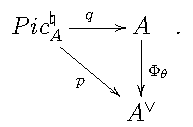
\includegraphics[width=0.1553\paperwidth]{images/L17-p144-polarization.pdf}\end{equation}\end{figure}
通过$p\times\mathrm{id}_A$，将Poincaré线丛拉回到$\operatorname{Pic}_A^\natural\times A$，得到线丛$\widetilde{\mathcal P}$及其万有相对平坦联络
\[\widetilde\nabla:\widetilde{\mathcal P}\longrightarrow\operatorname{pr}_A^*\Omega_A^1\otimes\widetilde{\mathcal P},\]
其中$\operatorname{pr}_A$、$\operatorname{pr}_\natural$分别为到$A$、到$\operatorname{Pic}_A^\natural$的投影。
在代数凝聚范畴中，定义Fourier--Mukai变换\znote{给定概形 $X,Y$ 与核 $K\in D^b_{\mathrm{coh}}(X\times Y)$，Fourier--Mukai 变换为 $\Phi_K(E)=\mathrm Rq_*(p^*E\overset{\mathrm L}{\otimes}K)$，其中 $p,q$ 为 $X\times Y$ 到 $X,Y$ 的投影。它是 Radon 变换在导出范畴中的公理化版本：核可取结构层、Poincaré 线丛等。Mukai 以 $K=\mathcal P$ 证明了 $D^b(X)\cong D^b(X^\vee)$，这正是一维几何 Langlands 对应的原型。当 $X,Y$ 为阿贝尔簇、核取 Poincaré 线丛时，$\Phi_K$ 是导出范畴的等价，即 Mukai 对偶；核的一般选取只使 $\Phi_K$ 成为函子。[来源：nLab "Fourier-Mukai transform"，\url{https://ncatlab.org/nlab/show/Fourier-Mukai+transform}（Last revised 2025-10-21；2026-11-14 访问）。]}$\mathfrak F_A$和$\mathfrak F_\natural$如下：
\[\mathfrak F_A:D_{\mathrm{coh}}^b(\mathcal D_A)\longrightarrow D_{\mathrm{coh}}^b(\OO_{\operatorname{Pic}_A^\natural}),\]
\[\mathfrak F_A(\mathcal K^\bullet):=\mathrm R(\operatorname{pr}_\natural)_*\operatorname{DR}_{\operatorname{Pic}_A^\natural\times A/\operatorname{Pic}_A^\natural}\bigl((\widetilde{\mathcal P},\widetilde\nabla)\overset{\mathrm L}{\otimes}\operatorname{pr}_A^*\mathcal K^\bullet\bigr).\]
这里，对光滑满射$Y\to S$，$\operatorname{DR}_{Y/S}$为相对de Rham复形，参见\lref{L14}，定义为
\[\operatorname{DR}_{Y/S}(\mathcal F^\bullet):=\omega_{Y/S}\overset{\mathrm L}{\otimes}_{\mathcal D_{Y/S}}\mathcal F^\bullet,\]
另一个变换为
\[\mathfrak F_\natural:D_{\mathrm{coh}}^b(\OO_{\operatorname{Pic}_A^\natural})\longrightarrow D_{\mathrm{coh}}^b(\mathcal D_A),\]
\[\mathfrak F_\natural(\mathcal K^\bullet):=\mathrm R(\operatorname{pr}_A)_*\bigl((\widetilde{\mathcal P},\widetilde\nabla)\overset{\mathrm L}{\otimes}_{\OO_{\operatorname{Pic}_A^\natural\times A}}\operatorname{pr}_\natural^*\mathcal K^\bullet\bigr).\]
\originalnumber{1}
\begin{theorem}\label{L17S2O1}
有以下典范的函子同构：
\[\begin{aligned}
\mathfrak F_\natural\circ\mathfrak F_A&\cong(-1)_A^*(\cdot)[-g(X)]&&\text{在 }D_{\mathrm{coh}}^b(\mathcal D_A)\text{上},\\
\mathfrak F_A\circ\mathfrak F_\natural&\cong(-1)_{\operatorname{Pic}_A^\natural}^*(\cdot)[-g(X)]&&\text{在 }D_{\mathrm{coh}}^b(\OO_{\operatorname{Pic}_A^\natural})\text{上}.
\end{aligned}\]
其中，对群概形$G$，$(-1)_G:G\to G$为将每个元素送到其逆元的态射。
\end{theorem}
\sourcepage{145}
现在取支撑于$p\in\operatorname{Pic}_A^\natural$的摩天层\znote{对闭点 $p\in S$，以 $p$ 为支撑的\textbf{摩天层}是 $i_{p*}\C$（其 $\OO_S$-模版本记为 $\OO_p$），其中 $i_p:\{p\}\hookrightarrow S$ 为嵌入；它在 $p$ 以外的茎全为零，在 $p$ 处的茎为 $\C$。摩天层是凝聚层导出范畴的一组紧生成元，其 Fourier--Mukai 像给出 $\mathcal D$-模，因而成为几何 Langlands 对应的基本构件。由于它只有一个非零茎，$\OO_p$ 还是 $\mathcal D$-模一侧最小、最易计算的构件。[来源：nLab "skyscraper sheaf"，\url{https://ncatlab.org/nlab/show/skyscraper+sheaf}（Last revised 2016-06-23；2026-11-14 访问）。]}$\OO_p$；$p=(L,\delta)$通过上述对应表示$X$上的线丛及其平坦联络。则
\[\mathfrak F_\natural(\OO_p)=\bigl(\widetilde{\mathcal P}|_{\{p\}\times A},\widetilde\nabla|_{\{p\}\times A}\bigr)\]
为$\mathcal D_A$模，恰是在几何Langlands对应下与$(L,\delta)$相对应的对象。从这一角度看，Langlands对应是Fourier--Mukai变换的一个特殊情形。此外，摩天层是有限支撑凝聚层的一族基本构件；相应的Hecke特征层可以看作这一子范畴的Fourier--Mukai像的基本构件。\idx{摩天层}
\section{\texorpdfstring{$\operatorname{Jac}(X)$上的行列式线丛}{Jac(X)上的行列式线丛}}\label{L17S3}\idx{行列式线丛}\idx{主极化}
我们要找到适当的线丛$\theta$，使\eqref{L17eq22}的三角交换。

设$\alpha:X\to B$为从曲线到阿贝尔簇的非常值态射，$B^\vee$为对偶阿贝尔簇，$\mathcal P_B$为$B^\vee\times B$上的Poincaré线丛。对$X$上的凝聚层$\mathcal F$，考虑其Fourier变换
\[\mathfrak F_{B^\vee}(\mathcal F):=\mathrm R(\operatorname{pr}_{B^\vee})_*\bigl(\operatorname{pr}_B^*\mathrm R\alpha_*\mathcal F\overset{\mathrm L}{\otimes}\mathcal P_B\bigr),\]
并将它视为$B^\vee$上凝聚层的Grothendieck群$K(B^\vee)$中的元素。该元素实际上属于由局部自由层生成的子群$K^0(B^\vee)$，因而可以定义与$\mathcal F$相关的行列式线丛$S(\mathcal F):=\det(\mathfrak F_{B^\vee}(\mathcal F))$。

映射$\mathcal F\mapsto S(\mathcal F)$给出从$X$上凝聚层的Grothendieck群$K(X)$到$\operatorname{Pic}_{B^\vee}$的群同态。特别地，
\[\begin{aligned}
S\bigl(\OO_X(\textstyle\sum_i n_ip_i)\bigr)&\cong S(\OO_X)\otimes\bigotimes_iS(\OO_{p_i})^{\otimes n_i}\\
&\cong S(\OO_X)\otimes\bigotimes_i(\mathcal P_B|_{\alpha(p_i)})^{\otimes n_i}.
\end{aligned}\]
因此得到映射
\[\operatorname{Div}(X)\longrightarrow\operatorname{Pic}_{B^\vee}^0\cong B,\qquad\sum_i n_ip_i\longmapsto\bigotimes_i(\mathcal P_B|_{\alpha(p_i)})^{\otimes n_i}.\]
它经由$\operatorname{Div}(X)\to\operatorname{Pic}_X$分解，故给出$\alpha_*:\operatorname{Pic}_X\to\operatorname{Pic}_{B^\vee}^0\cong B$。
\originalnumber{1}
\begin{proposition}\label{L17S3O1}
设$L$为$X$上的线丛。由行列式线丛的逆$S(L)^{-1}\in\operatorname{Pic}_{B^\vee}$按\eqref{L17eq21}诱导的映射$\Phi_{S(L)^{-1}}:B^\vee\to B$，等于复合
\[B^\vee\cong\operatorname{Pic}_B^0\xrightarrow{\alpha^*}\operatorname{Pic}_X^0\xrightarrow{\alpha_*}\operatorname{Pic}_{B^\vee}^0\cong B.\]
\end{proposition}
% [Tutor Note: 原书 p145 的命题 3.1 作 $\Phi_{S(L)}:B^\vee\to B$，由行列式线丛 $S(L)\in\operatorname{Pic}_{B^\vee}$ 诱导；译文按 $\Phi_{S(L)^{-1}}$ 处理，以与本节下文 $\Phi_{S(L)^{-1}}=\alpha_*$ 的复合方向一致。]
\sourcepage{146}
现在令$B=A^\vee$，其中$A=\operatorname{Jac}(X)$。固定$p_0\in X$，则$X\times A$上有唯一的归一化Poincaré线丛$\mathcal P_X$，满足$\mathcal P_X|_{\{p_0\}\times A}\cong\OO_A$。族$\mathcal P_X$诱导分类映射$\alpha:X\to B$。由于$\mathcal P_X\cong(\alpha\times\mathrm{id}_A)^*\mathcal P_B$，映射$\alpha^*:\operatorname{Pic}_B^0\to\operatorname{Pic}_X^0$在$A\cong\operatorname{Pic}_B^0\cong\operatorname{Pic}_X^0$的识别下是恒等映射。因此，由\eref{命题}{L17S3O1}，$\Phi_{S(L)^{-1}}=\alpha_*$。

另一方面，若$g(X)\ge1$，有嵌入
\begin{equation}\tag{3.1}\label{L17eq31}i:X\hookrightarrow A,\qquad p\longmapsto\OO_X(p-p_0).\end{equation}
容易看出$i_*:\operatorname{Pic}_X^0\to A$为恒等映射，而$i^*$为$\alpha_*$的逆。以$S_A(L_0)$表示通过映射$i:X\to A$得到的通常Fourier变换$F_A(L_0)\in K(A)$的行列式线丛。由Deligne关于阿贝尔Langlands对应的几何证明，有：
\originalnumber{2}
\begin{proposition}\label{L17S3O2}
对$X$上的任意线丛$L_0$，令$\theta:=S_A(L_0)\in\operatorname{Pic}_A$，$\theta':=S(L_0)\in\operatorname{Pic}_{A^\vee}$。则下列三角交换，且$\Phi_{\theta'}$为$\Phi_\theta$的逆同构\znoteplain{（上下文推断，无外部依据）本讲的 $\theta$ 与经典 theta 除子 $\OO(\Theta)$ 相差一个逆：经典叙述里 $\OO(\Theta)$ 丰沛、$\Theta=\{L:H^0(L\otimes L_0)\ne0\}$，而注记 3.3 说 $\theta^{-1}$ 丰沛且有在 $\{L:H^0(L\otimes L_0)\ne0\}$ 上消失的截面，两者正好互为逆。故命题 3.2 的三角与注记 3.3 的丰沛方向均以原书为准，读文献时需按各自约定换算。}：
\begin{figure}[H]\centering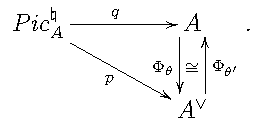
\includegraphics[width=0.2196\paperwidth]{images/L17-p146-dualpolarization.pdf}\end{figure}
\end{proposition}
% [Tutor Note: 原书 p146 的命题 3.2 作 $\theta'=S(L_0)\in\operatorname{Pic}_B$、$\theta=S_A(L_0)\in\operatorname{Pic}_A$（其中 $B=A^\vee$），而注记 3.3 又作 $\theta^{-1}$ 为丰沛线丛。原书未定义 $S(L_0)$、$S_A(L_0)$ 中取逆的约定，属约定不明而非笔误；译文照原文直译（$\theta=S_A(L_0)$、$\theta'=S(L_0)$），见命题 3.2 后的译者按。]
\begin{proof}
设$(L,\delta)$为$X$上带平坦联络的线丛。由Langlands对应，在$\operatorname{Pic}_X$上有带平坦联络的线丛$(\mathcal E,\nabla)$，满足$L\cong i^*\mathcal E$，其中$i$由\eqref{L17eq31}定义。
\end{proof}
\originalnumber{3}
\begin{note}[L17S3O3]
若$L_0$的次数为$g(X)-1$，则$\theta^{-1}=S_A(L_0)^{-1}$为丰沛线丛，并具有一个在相差非零常数倍的意义下唯一的截面。该截面恰好在满足$H^0(X,L\otimes L_0)\ne0$的点$L\in\operatorname{Pic}_X^0$处消失。
% [Tutor Note: 原书 p146 的注记 3.3 作 "$\theta^{-1}$ is an ample line bundle"；按命题 3.2 的直译 $\theta=S_A(L_0)\in\operatorname{Pic}_A$，此处即 $\theta^{-1}=S_A(L_0)^{-1}$。原书对取逆约定不明，译文照原文处理，见命题 3.2 后的译者按。]
\end{note}
\needspace{5\baselineskip}\section{第17讲参考文献}\label{L17S4}
\begin{references}
\refitem{L17bibL}{L} G. Laumon, \emph{Transformation de Fourier généralisée}, arXiv e-prints: \href{https://arxiv.org/abs/alg-geom/9603004}{alg-geom/9603004}.
\refitem{L17bibR}{R} M. Rothstein, \emph{Connections on the total Picard sheaf and the KP hierarchy}, Acta Applicandae Mathematicae 42 (1996) 297--308.
\sourcepage{147}
\end{references}
\needspace{4\baselineskip}关于平坦联络的命题：
\begin{references}
\refitem{L17bibP}{P} F. Pham, \emph{Singularités des systèmes différential de Gauss-Manin}, Progr. in Math. 2, Birkhäuser Verlag (1979).
\end{references}
